\documentclass[a4paper]{scrartcl}
\usepackage[ngerman]{babel}
\usepackage{amsmath,amssymb,amsthm,amsfonts,amsbsy,latexsym}
\usepackage[utf8]{inputenc}
\usepackage[T1]{fontenc}
\usepackage{enumerate,url}
\usepackage{graphicx}
 \usepackage{float}		% Erzwingen der Position einer Grafik mittels Option[H]
\usepackage{bibgerm}
\usepackage[babel,german=guillemets]{csquotes}
\usepackage{biblatex}	% Einbinden von biblatex zur Literaturverwaltung
\addbibresource{literaturelibrary/literatureLib.bib}	% Literatursammlung

\usepackage[printonlyused]{acronym}	% Abkürzungsverzeichnis

%\usepackage[style=numeric-comp]{biblatex}
\usepackage{listings}
%\usepackage[svgnames]{xcolor}

 \usepackage{blindtext} %  Lorem ipsum - Text "Fülltext"

\usepackage{listings}		% Quelltext verwenden
\usepackage{fancybox}  	% Box um Formel
\usepackage{varwidth}
\usepackage{lscape}
\usepackage{verbatim}	% mehrzeiliger Kommentar
\usepackage{titleref}	% Verweis auf Kapitel mit Titel
\usepackage{listings}	% Einbinden von Quelltext
\usepackage{color}		% Einfärben von Quelltext

\definecolor{mygreen}{rgb}{0,0.6,0}
\definecolor{mygray}{rgb}{0.5,0.5,0.5}
\definecolor{mymauve}{rgb}{0.58,0,0.82}

\lstset{ %
  backgroundcolor=\color{white},   % choose the background color; you must add \usepackage{color} or \usepackage{xcolor}
  basicstyle=\footnotesize,        % the size of the fonts that are used for the code
  breakatwhitespace=false,         % sets if automatic breaks should only happen at whitespace
  breaklines=true,                 % sets automatic line breaking
  captionpos=b,                    % sets the caption-position to bottom
  commentstyle=\color{mygreen},    % comment style
  deletekeywords={...},            % if you want to delete keywords from the given language
  escapeinside={\%*}{*)},          % if you want to add LaTeX within your code
  extendedchars=true,              % lets you use non-ASCII characters; for 8-bits encodings only, does not work with UTF-8
  frame=single,	                   % adds a frame around the code
  keepspaces=false,                % keeps spaces in text, useful for keeping indentation of code (possibly needs columns=flexible)
  keywordstyle=\color{blue},       % keyword style
  language=Octave,                 % the language of the code
  otherkeywords={*,...},           % if you want to add more keywords to the set
  numbers=left,                    % where to put the line-numbers; possible values are (none, left, right)
  numbersep=5pt,                   % how far the line-numbers are from the code
  numberstyle=\tiny\color{mygray}, % the style that is used for the line-numbers
  rulecolor=\color{black},         % if not set, the frame-color may be changed on line-breaks within not-black text (e.g. comments (green here))
  showspaces=false,                % show spaces everywhere adding particular underscores; it overrides 'showstringspaces'
  showstringspaces=false,          % underline spaces within strings only
  showtabs=false,                  % show tabs within strings adding particular underscores
  stepnumber=2,                    % the step between two line-numbers. If it's 1, each line will be numbered
  stringstyle=\tiny\color{mygreen},     % string literal style
  tabsize=2,	                   % sets default tabsize to 2 spaces
  title=\lstname                   % show the filename of files included with \lstinputlisting; also try caption instead of title
}


% /===========================================================================\
%
%   Anfang vom Dokument
%
% \===========================================================================/

\begin{document}

\renewcommand\lstlistingname{Quellcode}	% Setzt die Quellcodebezeichnung(Aufzählung) Quellcode 1,2,3,4,...n
% /===========================================================================\
%
%   Titelseite
%
% \===========================================================================/
\thispagestyle{empty}

\begin{center}
\Large{Hochschule für Technik und Wirtschaft Berlin (HTW)}\\
\end{center}
 
 
\begin{center}
\Large{Fachbereich IV - Informatik, Kommunikation und Wirtschaft}
\end{center}
\begin{verbatim}


\end{verbatim}
\begin{center}
\textbf{\LARGE{Dokumentation}}
\end{center}
\begin{verbatim}
 
 
\end{verbatim}
\begin{center}
\textbf{im Studiengang Angewandte Informatik}
\end{center}
\begin{verbatim}
\end{verbatim}
 
\begin{flushleft}makeindex %.nlo -s nomencl.ist -o %.nls
\begin{tabular}{lll}
\textbf{Fach:} & & Entwicklung von Multimediaanwendungen\\
& & \\
& & \\
\textbf{Thema:} & & Sogo\\
\textbf{Bschreibung:}& & Viergewinnt im dreidimensionalen Raum (3D) \\
& & \\
& & \\
\textbf{eingereicht von:} & & Nils Brandt, 549906 \\
& & Alexander Lüdke, 548965 \\
& & \\
\textbf{eingereicht am:} & &  Sommersemester 2016 \\
& & \\
& & \\
\textbf{Dozenten:} & & Sebastian Bauer \\
& & 	Sebastian Keppler
\end{tabular}
\end{flushleft}

\newpage

% /===========================================================================\
%
%   Inhaltsverzeichnis
%
% \===========================================================================/
\thispagestyle{empty}

\tableofcontents

\newpage

% /===========================================================================\
%
%   Hauptdokument
%
% \===========================================================================/

\setcounter{page}{3}

% /===========================================================================\
%   Einleitung
% \===========================================================================/
\section{Einleitung}\label{ch:Einleitung}
Die Applikation Sogo stellt den Komplettbeleg für das Fach Entwicklung von Multimediaanwendungen dar. Hierbei lag der Fokus sowohl auf der Funktionalität der Applikation als auch auf das Erarbeiten, Planen und Implementieren des Softwareprojektes. Dieses Projekt stellt zum gegenwärtigen Zeitpunkt, im vierten Semester des Studienfachs AI, das größte Softwareprojekt dar, welches als Beleg abzugeben ist.
\\
Die Grenzen der Realisierung sind weit gefasst, da sie zum Einen durch die Team-Mitglieder und zum Anderen durch die Dozenten mittels Anforderungen festgelegt wurden. Die Hauptimplementierung soll mit der Klassen-Bibliothek Qt, auf Basis von C++ erfolgen.

% /===========================================================================\
%   Grundlagen
% \===========================================================================/
\section{Grundlagen}\label{ch:Grundlagen}
% Beschreibung des Spiels
Für unser Projekt haben wir uns für das Spiel Sogo entschieden, welches auch unter dem Namen Raummühle, 3D-Mühle oder Vier gewinnt Professional bekannt ist. Dabei gilt es wie auch im zweidimentsionalen Raum, seine Spielsteine direkt nebeneinander in der Horizontalen sowie in der Vertikalen zu platzieren und damit, je nach Spielfeldgröße, eine durchgehende Linie zu besetzten. In Sogo muss zusätzlich die dritte Dimension beachtet werden, in der es möglich ist, seine Seine diagonal und horizontal im Raum zu platzieren, was die Komplexität und damit den Schwierigkeitsgrad erhöht.
\\
Die Spielfeldgröße ist im Grundaufbau ein 4x4x4 Würfel, welchen wir für unsere Applikation auf 5x5x5 und 3x3x3 erweitert haben. 
Jeder Spieler verfügt im Raster
	\begin{itemize}
		\item 3x3x3 über 13 Spielsteine
		\item 4x4x4 über 32 Spielsteine		
		\item 5x5x5 über 62 Spielsteine
	\end{itemize}
Um sich innerhalb des Spielbrettes zu orientieren wird für die jeweilige Spielfeldgröße ein Raster festgelegt, welches sich wie folgt zusammensetzt. 
Für das Spielfeld
\begin{itemize}
		\item 3x3x3 wird die Grundfläche von ein bis neun und die Ebenen von 		eins bis drei durchnummeriert. Daraus folgt die Notation \\ $\mathcal{M}=\{(1,1),(1,2),(1,3),...(9,3)\}$.
		\item 4x4x4 gibt es die Möglichkeit die Grundfläche in Hexadezimal-Notation und die Ebenen von eins bis vier aufzuteilen. Daraus folgt die Notation \\
$\mathcal{M}=\{(1,1),(2,1),(3,1),...(F,4)\}$.
		\item 5x5x5 wird das bekannte Schachraster verwendet welches die Grundfläche von A-E und eins bis fünf sowie die die Ebenen von eins bis fünf festlegt. Daraus folgt die Notation \\
$\mathcal{M}=\{(A,1,1),(A,2,1),(A,3,1),...(E,5,5)\}$.
	\end{itemize}
	
Der grundlegende Spielverlauf ergibt sich wie folgt. Zuerst wird festgelegt, wer welche Spielsteinfarbe erhält und wer das Spiel beginnen darf. Anschließend stecken/setzen beide Spieler ihre Spielsteine auf den Stab der jeweiligen Position. Gewonnen hat der Spieler, der seine Spielsteine in einer Linie senkrecht, waagerecht, diagonal in einer Ebene oder diagonal nach oben bzw. unten gesetzt hat. Insgesamt sind 76 Möglichkeiten gegeben zu gewinnen, wobei auch ein unentschieden möglich ist. Dies geschieht, wenn alle Spielsteine von beiden Spielern gesetzt sind und keiner eine Linie mit seinen Spielsteinen besetzen konnte.

% /===========================================================================\
%   Analyse
% \===========================================================================/
\section{Analyse}\label{ch:Analyse}

%Quellverweis - Lektüre
% Use-Case
Wie zuvor im Kapitel ~\ref{ch:Einleitung} \glqq\titleref{ch:Einleitung}\grqq \ auf Seite \pageref{ch:Einleitung} beschrieben, sind die Grenzen der Realisierung sehr flexibel und mittels Anforderungen definiert, wobei wir in diesem Abschnitt nur auf die eingehen wollen, die unserer Meinung nach hervorzuheben sind und die von uns selber erfasst wurden.
\\
Die ersten Anforderungen waren schnell erfasst, weil wir uns an den Vorgaben der zur Verfügung gestellten Projekten orientierten, ohne zu wissen, wie der Aufwand einzuschätzen war, was Auswirkung auf das Ende des Projektes hatte. Doch dazu kommen wir im Abschnitt ~\ref{ch:Ergebnis} \glqq\titleref{ch:Ergebnis}\grqq \ auf Seite \pageref{ch:Ergebnis}. Betrachten wir nun eine kleine Auswahl der zu implementierenden Anforderungen. 
\\
\\
\textbf{Anforderung:} 
Die Größe des Spielfelds soll vor der Partie in der GUI konfigurierbar sein. Die Standardgröße ist 4x4x4, wobei die Möglichkeit zum 3x3x3 oder 5x5x5 ausgewählt werden kann. 3x3x3 oder 5x5x5 ausgewählt werden kann.
\\
\textbf{Beschreibung:} Das Spielfeld stellte die Grundlage für Sogo dar. Natürlich sollte es möglich sein die Spielfeldgröße auszuwählen. Als wir uns überlegten wie wir das Spielfeld organisieren sollten, kam uns der Gedanke das 5x5x5 Spielfeld variabel zu gestalten bzw. die Steine auf eine andere Art zu setzen. Wir konzipierten das Spielfeld so, dass die Grundfläche, nicht wie bei 4x4x4 und 3x3x3 unten liegt, sonder in der mittleren Schicht liegt also auf Ebene drei.  Dadurch war der Spieler in der Lage seine Steine sowohl von oben als auch von unten zu setzen. Nachdem wir im weiteren Verlauf der Entwicklung festgestellt hatten, dass die Implementierung des einfachen Spielfeldes schon sehr viel Zeit in Anspruch nahm, mussten wir diese Spieloption vorerst zurückstellen. Was dazu führte das in der Version 1.0 das Spielfeld 5x5x5 in der Standardkonfiguration gespielt werden kann.
\\ 
\\
\textbf{Anforderung:} 
Die aktuelle Spielhistorie wird für das laufende Spiel angezeigt.
\\ 
\textbf{Beschreibung:} Dies war uns wichtig, de es dem Spieler die Möglichkeit geben sollte, die bereits gespielten Züge nachvollziehen zu könne und sie bei Gelegenheit zu analysieren.
\\
\\
\textbf{Anforderung:} 
Beim Spiel Mensch gegen Computer soll es möglich sein, die Spielstärke des Computer aus drei Schwierigkeitsgraden auszuwählen.
\\
\textbf{Beschreibung:} Hierbei war ein Hauch von künstlicher Intelligenz zu erahnen, welchen wir nutzten, um den Minimax-Algorithmus zu implementieren, der die optimale Spielstrategie der AI festlegen sollte. Hierzu betrachten wir im Kapitel ~\ref{ch:AI} \glqq\titleref{ch:AI}\grqq \ auf Seite \pageref{ch:AI} den Quellcode der Implementierung.
\\
\\
\textbf{Anforderung:} 
Das Spiel ist sowohl in 2D- als auch in 3D-Ansicht spielbar/visualisierbar.
\\
\textbf{Beschreibung:} Diese Anforderung stellte einen immensen Arbeitsaufwand dar, der zuvor nicht einzuschätzen war. Hierzu müssen wir etwas weiter ausholen, da diese Anforderung nicht nur das Studienfach Entwicklung von Multimediaanwendungen sondern auch das Fach Computergrafik betraf. Wir hatten vor beide Fächer in einem Projekt zu vereinen. Im Fach Computergrafik mussten wir mit der Grafikbibliothek OpenGL(Open Graphics Library) eine 3D-Szene erstellen. Diese Szene sollte sowohl in 3D als auch interaktiv sein. Innerhalb der Vorlesung erstellten wir unter Visual Studio 2015 eine lauffähige Version von Sogo in 3D, was im Anschluss folgte, war \glqq lediglich\grqq \ die Überführung und Herstellung der Lauffähigkeit der 3D Ansicht in Verbindung mit einer bis dahin erstellten Spiellogik. Letztendlich brauchten wir, nur für die  Implementierung dieser Anforderung, vier Wochen. Was zum Einen mit der Überführung von OpenGL-Syntax in die Qt-Syntax zu tun hatte und zum Andern mit der OpenGL Version der einzelnen Systeme, welche für die Erstellung zum Einsatz kamen. Im Labor war es nur möglich unter Ubuntu Qt zu nutzen, was jedoch bedeutete eine alte Version von OpenGL zu verwenden, die mit der Implementierungsversion nicht kompatibel war. Die einzige Möglichkeit war, die komplette Umsetzung der 3D-Umgebung auf den heimischen Rechner zu realisieren.
\\ 
\\
Nachdem wir die Anforderungen ausformuliert hatten, legten wir uns ein Git-Repository an, welches wir für das Projekt verwendeten. Dieses wurde anfänglich genutzt um gemeinsame Dokumente wie den Anforderungsbericht und einen zentralen ToDo-Zettel zu verwalten, der als Projekttagebuch dienen sollte. In diesem Projekttagebuch legten wir fest wer welche Anforderung übernahm, wie der Status des Bearbeitung ist und welche zusätzlichen Arbeiten noch zu erledigen waren, die vorher nicht ersichtlich waren. Darüber hinaus nutzten wir ihn, um uns gegenseitig Zusatzinformation zukommen zu lassen, die uns während der eigenen Bearbeitung auffielen und die wir dem jeweils anderen mitteilen wollten. Der Hauptverwendungszweck lag definitiv auf der Versionierung unseres Quelltextes.

% /===========================================================================\
%   Entwurf
% \===========================================================================/
\section{Entwurf}\label{ch:Entwurf}

% Klassendiagramm

% /===========================================================================\
%   Implementation
% \===========================================================================/
\section{Implementierung}\label{ch:Implementierung}

% Das Raster der jeweiligen Spielfelder wurde vereinfacht auf Grund einfacher Physik, die Schwekraft. Daher ergibt sich für jedes Spiel feld eine Notation von (1,1)... (n,m).

% Verwendung von Code-Snipets

% core/
\subsection{Vector2}\label{ch:Vector2}
\subsection{Vector3}\label{ch:Vector3}
\subsection{Artificial Intelligence(AI)}\label{ch:AI}
\subsection{PlayingField}\label{ch:PlayingField}
\subsection{GameData}\label{ch:GameData}
\subsection{Player}\label{ch:Player}


% gui/
\subsection{Spielmenüs}\label{ch:Spielmenüs}
Die komplette Navigation der Applikation wurde mittels Qt implementiert. Hierzu legten wir zuvor fest, welchen Menüs benötigt werden, um den zuvor erstellten Anforderungen gerecht zu werden. Daraus resultierten die folgenden Menüs und Untermenüs. Generell waren wir von Anbeginn darauf fokussiert das Backend zu erstellen und das Frontend lediglich als funktionale Darstellung zu behandeln, was zur Folge hat, dass unsere Menüs nicht grafisch aufbereitet sind. Doch dieser Punkt wird im dem Kapitel ~\ref{ch:Ergebnis}  \glqq\titleref{ch:Ergebnis}\grqq \ auf Seite \pageref{ch:Ergebnis} aufgegriffen.
\\
Das interessante an den Menüs war, dass sie erst erstellt wurden, nachdem die Spiellogik und die Spielansicht erstellt wurde. Im Anschluss wurde nur noch auf die benötigten Objekte eingegangen, die die Spielansicht benötigte. D.h. um ein Spiel zu beginnen, musste das GameData-Objekt mit Werten befüllt werden, welche sich wiederum aus den Benutzereingaben generieren ließen, was letztendlich den Art der Eingaben und Ansicht der Spielmenüs beeinflusste. Auf diese wollten wir nun im folgenden Kapitel eingehen.

\subsubsection{StartMenu}\label{ch:StartMenu}
Sobald das Spiel gestartet wird, gelangt man in das Startmenü. Hier hat man wie in der Abbildung~\ref{fig:Startmenü}: auf der Seite \pageref{fig:Startmenü} zu sehen ist, folgende Auswahlmöglichkeiten.

\begin{itemize}
	\item \textbf{Sprache - [en-gb]} Wechselt die Sprache von deusch nach englich und umgekehrt.
	\item \textbf{Fullscrenn} Wechselt in den Vollbildmodus und wieder zurück in den Fenstermodus.
	\item \textbf{Neue Partie} Öffnet das NewSessionMenü, welches die Einstellungen für ein neues Spiel beinhaltet.
	\item \textbf{Load} Hierbei wird das letzte Spiel geladen, welches gespeichert wurde.
	\item \textbf{Bestenliste} Hier sollte eine Bestenliste angezeigt werden, deren Darstellung nicht realisiert wurde. Doch darauf gehen wir im Kapitel \ref{ch:Ergebnis} auf der Seite \pageref{ch:Ergebnis} weiter ein.
	\item \textbf{Ende} Damit wird die komplette Anwendung beendet.
\end{itemize}

\begin{figure}[H]
 \centering
 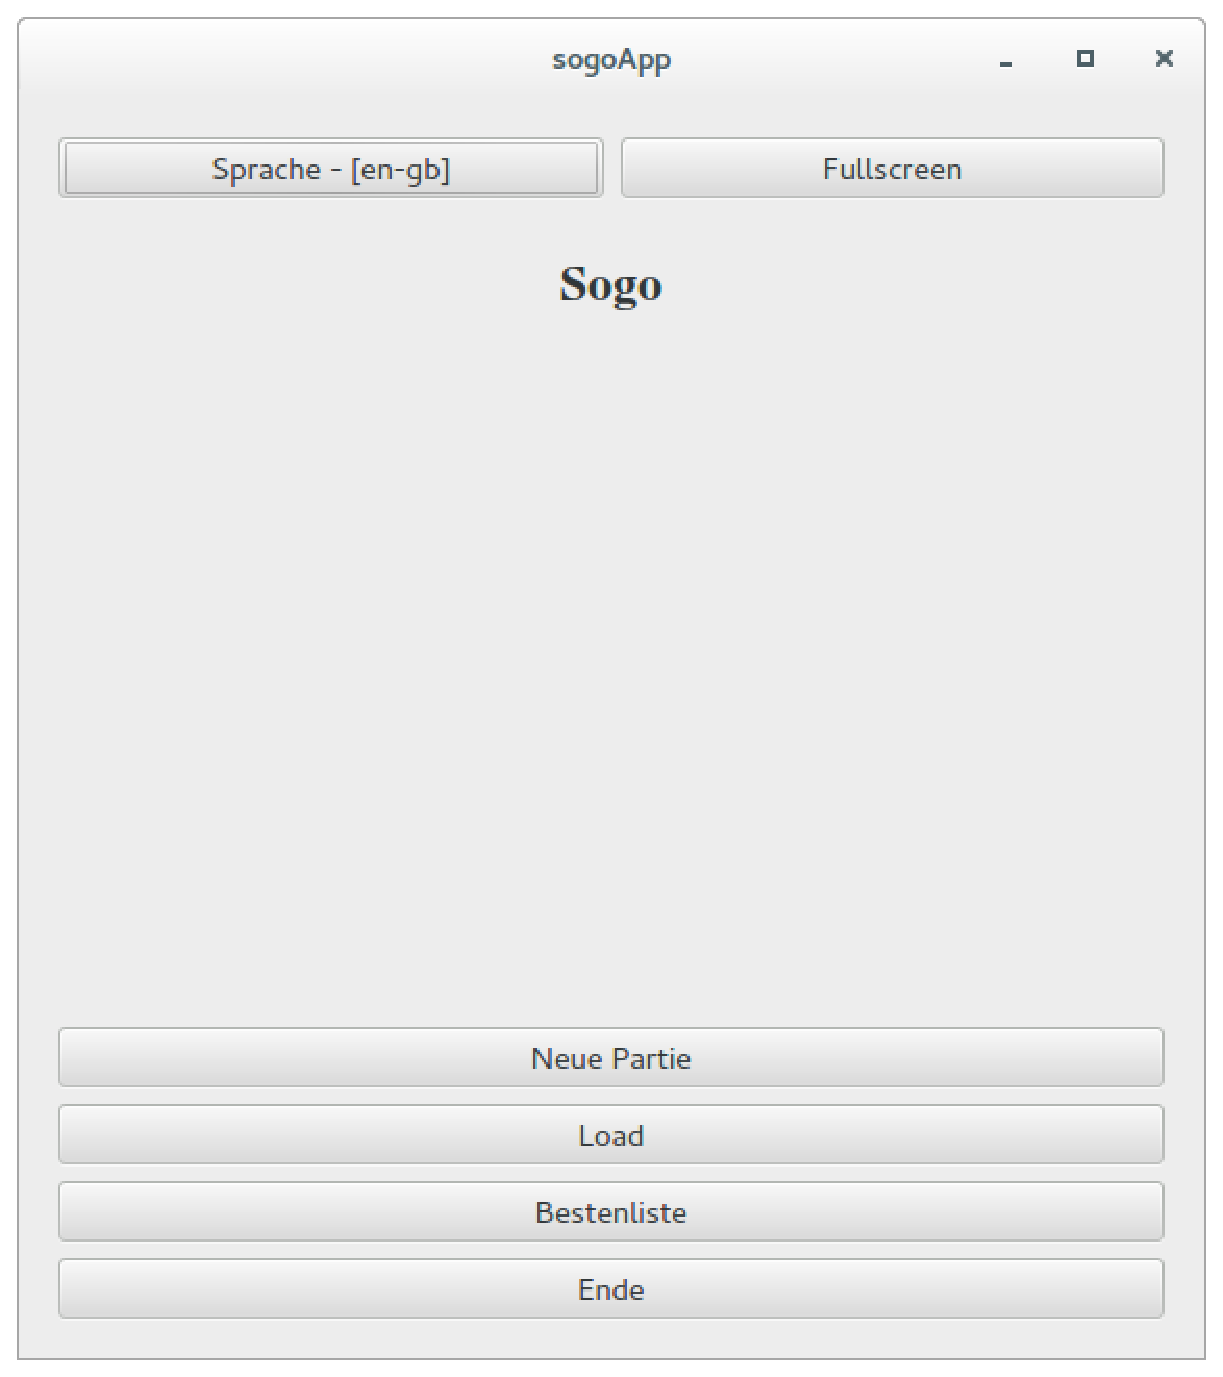
\includegraphics[scale=0.35]{graphics/startmenu.eps}
 \caption{Das Startmenü}
 \label{fig:Startmenü}
\end{figure}

\subsubsection{NewSessionMenu}\label{ch:NewSessionMenu}
Nachdem die Auswahl getroffen wurde eine neues Spiel zu beginnen, gelangt man in das NewSessionMenü, welches die grundlegende Spielkonfiguration für die folgende Partie festlegt. Die Konfigurationsmöglichkteiten werden durch die Abbildung~\ref{fig:NewSessionmenü} auf der Seite \pageref{fig:NewSessionmenü} dargestellt und im Folgenden kurz beschrieben. 

\begin{itemize}
	\item \textbf{Sprache - [en-gb]} Wechselt die Sprache von deusch nach englich und umgekehrt.
	\item \textbf{Fullscrenn} Wechselt in den Vollbildmodus und wieder zurück in den Fenstermodus.
	\item \textbf{Spieler1} Hier kann der Name des ersten Spielers eingegeben werden, der wenn keiner eingegeben wird standardmäßig Spieler1 lautet.
	\item \textbf{Spielfeldgröße} Hier wird die Spielfeldgöße festgelegt, welches im Standardspiel 4x4x4 ist.
	\item \textbf{Modus} Über diese Option wird die Art des Spiels festgelegt. Wobei PvC für Player vs. Computer, PvP(lokal) für Player vs. Player am lokalen Rechner und PvP(Netzwerk) für Player vs. Player im Netzwerk steht. Wobei die Netzwerkkomponenten nicht implementiert wurde, was im Kapitel \ref{ch:Ergebnis} auf Seite \pageref{ch:Ergebnis} näher erläutert wird.
	\item \textbf{\glqq Schwierigkeitsgrad\grqq} Dieser wurde mit einer Steigerung von ein(einfach) bis drei(schwer) versehen, wobei diese Optionen in der momentanen Implementierung für geübte Spieler keine Herausforderung darstellt. Hierzu müsste man die Tiefe der Berechnung des MiniMax-Algorithmus aus dem Kapitel \ref{ch:AI} anpassen.
	\item \textbf{Spiel starten} Das Spiel mit der momentan gesetzten Konfiguration starten.
	\item \textbf{Ende} Damit wird die komplette Anwendung beendet.
\end{itemize}

Eine Besonderheit, die sich durch das ganze Projekt zog, war die Strukturierung des Frontends mittels Qt. Das soll heißen, dass jedes grafische Objekt verschachtelt und in ein Label, Widget und Layout verpackt wurde, was letztendlich dazu führte, dass die Anzahl der Attribute einer Klasse, an Komplexität zunahmen, wobei sich die Interaktionsmöglichkeiten des Benutzers nur geringfügig veränderten.
 
\begin{figure}[H]
 \centering
 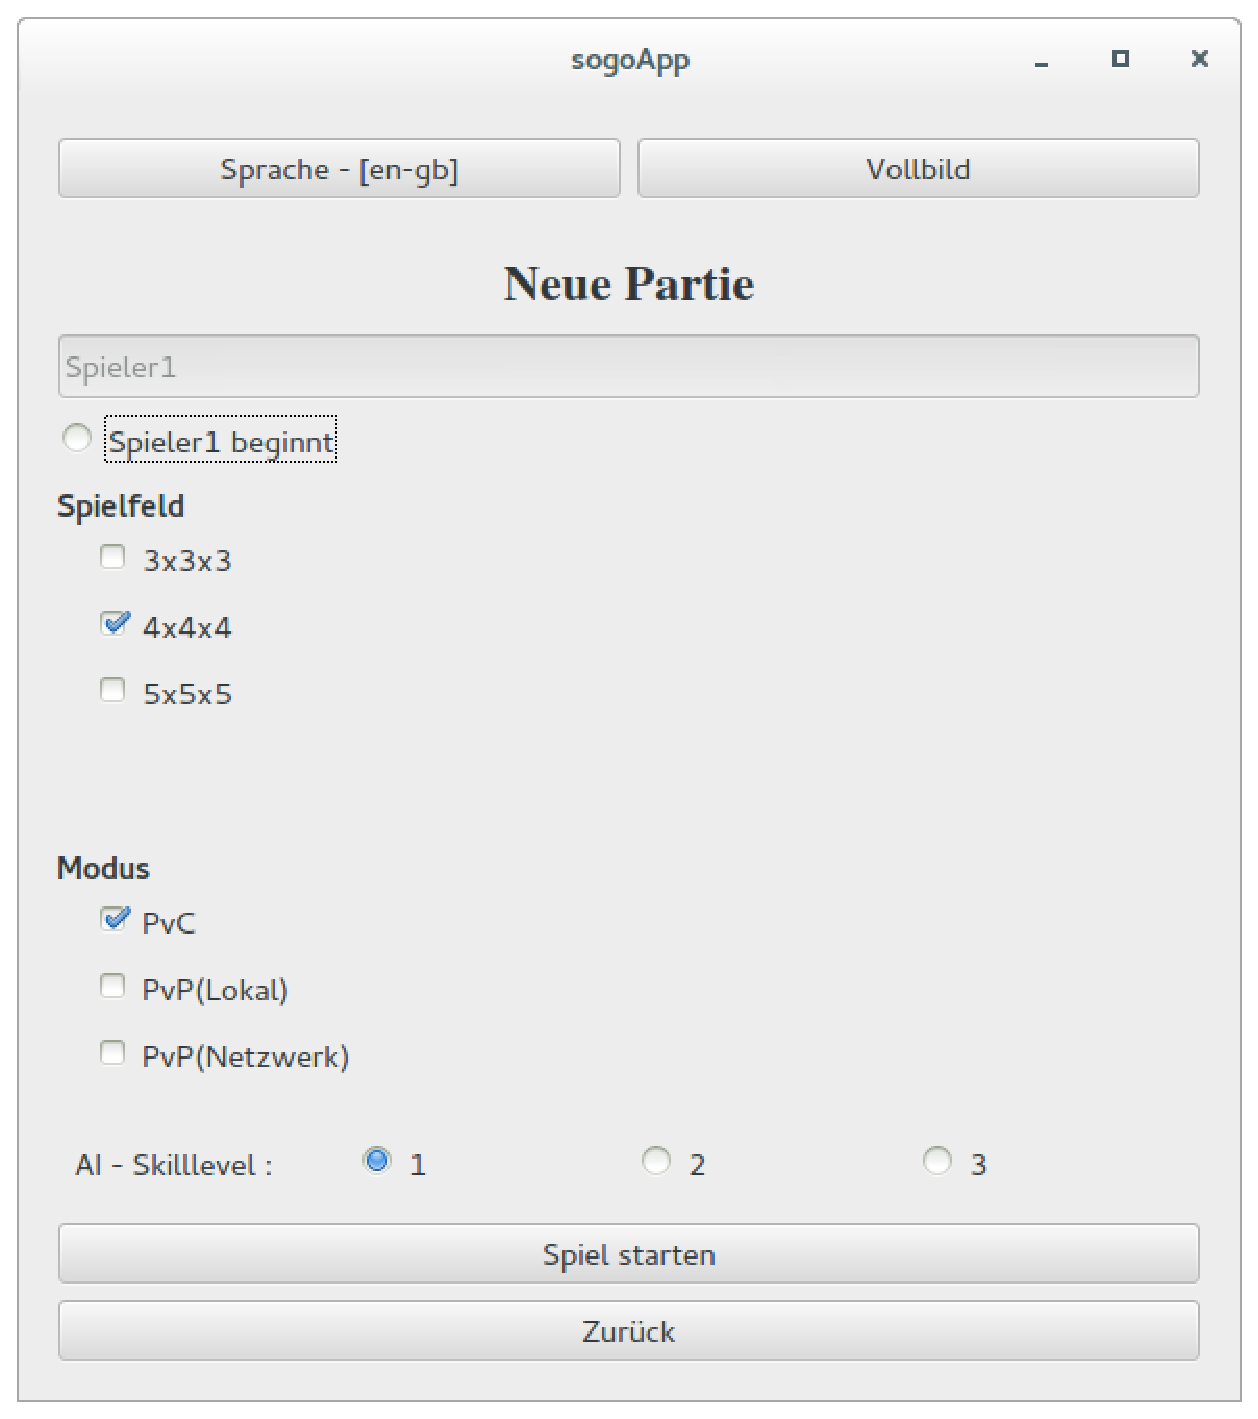
\includegraphics[scale=0.35]{graphics/newsession.eps}
 \caption{Das NewSessionmenü}
 \label{fig:NewSessionmenü}
\end{figure}

\begin{comment}
	\subsubsection{HighscoreMenu}\label{ch:HighscoreMenu}
	\begin{figure}[H]
	 \centering
	 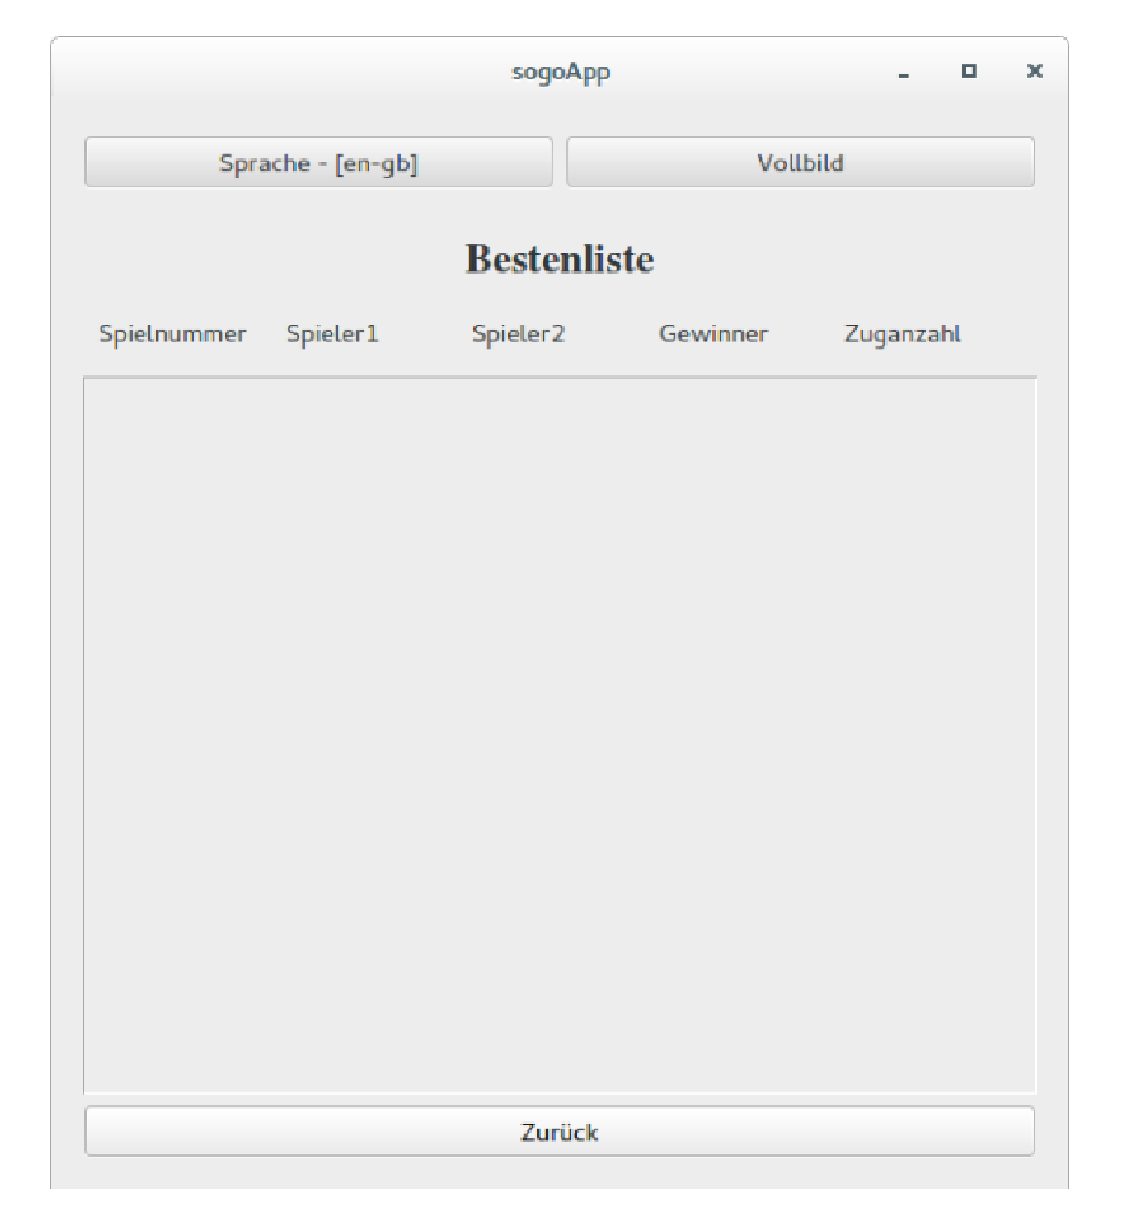
\includegraphics[scale=0.35]{graphics/highscore.eps}
	 \caption{Das Highscoremenü}
	 \label{fig:Highscoremenü}
	\end{figure}
\end{comment}

\subsubsection{PauseMenu}\label{ch:PauseMenu}
\begin{figure}[H]
 \centering
 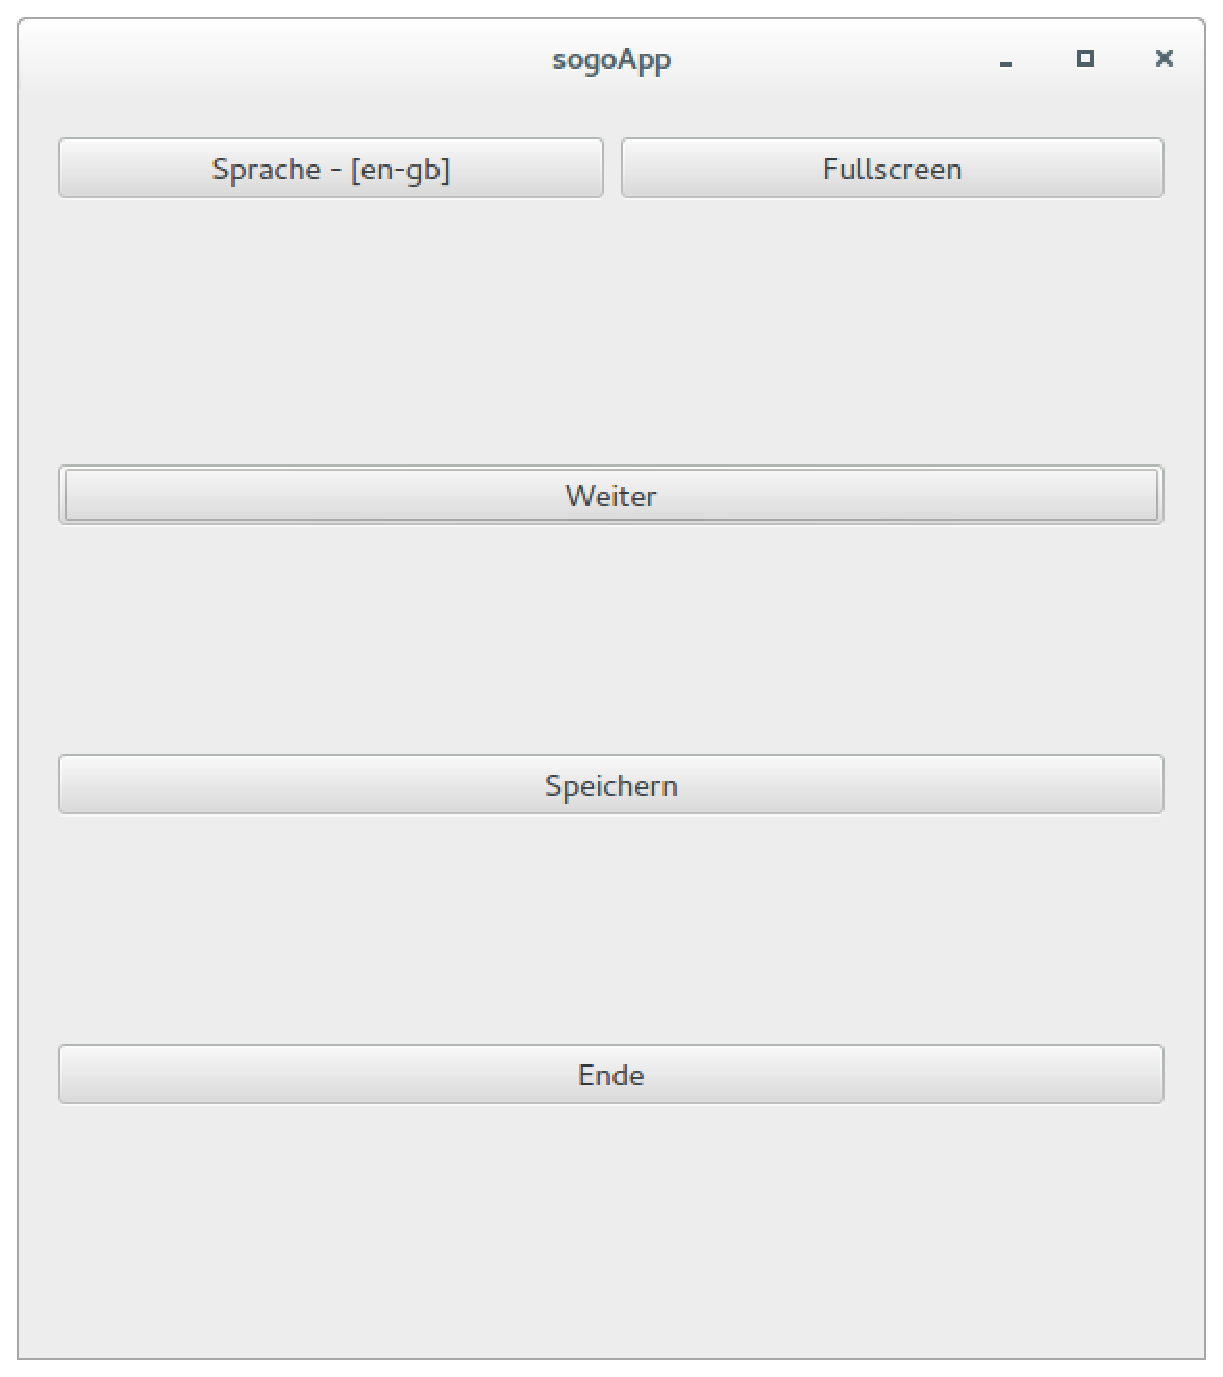
\includegraphics[scale=0.35]{graphics/pausemenu.eps}
 \caption{Das Pausemenü}
 \label{fig:Pausemenü}
\end{figure}

\subsubsection{Sprache}\label{ch:Sprache}
Ein Entscheidendes Kriterium war die Möglichkeit die Sprache zu jedem Zeitpunkt zu wechseln. Hierzu entschieden wir uns, die zwei, aus unserer Sicht, nützlichsten Sprachen zu wählen, nämlich deutsch und englisch. Dazu nutzten wir die Implementierung eines Translators. Hierzu wurden zwei erstellte .qm-Dateien den Ressourcen hinzugefügt, die die Übersetzung der einzelnen Textbausteine beinhalteten. Um ein derartiges Wörterbuch zu erstellen, mussten sämtliche String-Texte, wie exemplarisch im Quellcodeausschnitt Quellcode~\ref{lst:Translatortext}: auf Seite \pageref{lst:Translatortext} dargestellt ist, formatiert werden. 

\begin{lstlisting}[caption={Translatortext}\label{lst:Translatortext},captionpos=t]
     m_playGameButton = new QPushButton(tr("Start Game"));
\end{lstlisting}
Die tr-Funktion gefolgt von dem Text, der übersetzt werden soll. 
\\
Damit eine Übersetzung einem Text zugeordnet werden kann, hat man die Möglichkeit die .gm-Dateien mittels Texteditor anzupassen, oder den hauseigenen Translatoreditor Linguist von Qt zu verwenden, wobei die zweite Variante sehr komfortabel ist.
\\ 
\\
Damit man innerhalb des Spiels die Sprache gewechselt werden kann muss für jede Ansicht ein zusätzliches Event implementiert werden, welches zuvor in der Klasse mainwindow definiert wurde. Die Implementierungen werden in den folgenden Quelltextausschnitten dargestellt.

\begin{lstlisting}[caption={Translator}\label{lst:Translator},captionpos=t]
void MainWindow::ChangeLanguage()
{
    qApp->removeTranslator(m_translator);
    delete(m_translator);
    m_translator = new QTranslator();
    if(m_languageEnglish)
    {
        if(m_translator->load(":/sprache/Translations/sogoapp_de.qm"))
        {
            std::cout << "translator loaded" << std::endl;
        }
        else
        {
            std::cout << "translator did not load...whyever!!!" << std::endl;
        }
        m_languageEnglish = false;
    }
    else
    {
        if(m_translator->load(":/sprache/Translations/sogoapp_en.qm"))
        {
            std::cout << "translator loaded" << std::endl;
        }
        else
        {
            std::cout << "translator did not load...whyever!!!" << std::endl;
        }
        m_languageEnglish = true;
    }
    qApp->installTranslator(m_translator);

}
\end{lstlisting}
Hier werden die Sprachdateien geladen, die für die Übersetzung verantwortlich sind.

\begin{lstlisting}[caption={Sprachwechsel}\label{lst:Sprachwechsel},captionpos=t]
inline void changeEvent(QEvent *event)
    {
        if (event->type() == QEvent::LanguageChange) {
            m_newSessionButton->setText(tr("New Session"));
            m_highscoreButton->setText(tr(("Highscore")));
            m_exitButton->setText(tr("Exit"));

        } else
            QWidget::changeEvent(event);
    }
\end{lstlisting}
Anschließend wurde der Sprachwechsel mit einen Button im Frontend verknüpft und auf jeder Ansicht zugänglich gemacht.

\subsection{Mainwindow}\label{ch:Mainwindow}
\subsection{GameView}\label{ch:GameView}
\subsubsection{GameView2D}\label{ch:GameView2D}
\subsubsection{GameView3D}\label{ch:GameView3D}
\subsection{GameVisualizer}\label{ch:GameVisualizer}
\subsection{PlayerInput}\label{ch:PlayerInput}
\subsection{HistoryDisplay}\label{ch:HistoryDisplay}



%utility
\newpage
\subsubsection{Logger - Der hauseigene Debugger}\label{ch:Logger}
Dieses kleine Stück Quelltext, siehe unten stehendes Quellcode~\ref{lst:CodeLogger}: auf Seite \pageref{lst:CodeLogger}, welches uns dabei geholfen hat den Großteil der aufgetretenen Fehler ausfindig zu machen und zu beheben. Durch die zunehmende Komplexität des Projektes und der damit verbundenen Zunamen an Quelltext haben wir, hauptsächlich Herr Brandt, eine Möglichkeit geschaffen, den Quelltext in einzelne Abschnitte zu unterteilen und sie auf ihre Funktion zu überprüfen, um dadurch die Fehlerquelle ausschließen zu können. Dieses Stück Quelltext ist, in unseren Augen, ein ideales Beispiel für das Wiederverwenden von Quelltext in zukünftigen Projekten, wobei eine kontinuierliche Weiterentwicklung angestrebt werden sollte.
\lstinputlisting
    [caption={Logger - Debugger} 	% Titel
    	\label{lst:CodeLogger},			% Zum Referenzieren    
    emptylines=0,					% Zulassen der leeren Zeilen.(hier keine)
    captionpos=t,					% Titelanzeige on top(t)
    language=c++,					% Programmiersprache
    linerange={19-26,33-40,48-55,62-69,79-86}]%,98-110}]	% Auswahl Zeilen
{../../src/utility/Logger.cpp}		% Sourcefile
%external
\subsection{3D Umsetzung}\label{ch:3DUmsetzung}

% /===========================================================================\
%   Test
% \===========================================================================/
\section{Test}\label{ch:Test}
\subsection{Unit-Test}\label{ch:Unit}
\subsection{Valgrind}\label{ch:Valgrind}

% /===========================================================================\
%   Ergebnis
% \===========================================================================/
\section{Ergebnis}\label{ch:Ergebnis}
% Auswertung
% spartanisches Frontend - aus kap Spielmenü
% Realisierung der Highscoremenüs aus Kapitel Startmenü

\subsection{Vergleich}\label{ch:Vergleich}
\subsection{Zusammenfassung}\label{ch:Zusammenfassung}
\subsection{Bewertung}\label{ch:Bewertung}
\subsection{Ausblick}\label{ch:Ausblick}

\newpage

% /===========================================================================\
%
% 	Abkürzungsverzeichnis
%
% \===========================================================================/
\addsec{Abkürzungsverzeichnis}\label{sec:Abkürzungsverzeichnis}

\begin{acronym}%[längste Abkürzung für einen gleichmäßigen Abstand]

	% example
	\begin{comment}
	 	\acro{SQL}{Structured Query Language}
	 	\acro{Bash}{Bourne-again shell}
	 	\acro{JDK}{Java Development Kit}
		\acro{VM}{Virtuelle Maschine}
	 	\acro{I2C}[I²C]{Inter-Integrated Circuit}
 	\end{comment}
 	
 	\acro{bofh}{Bastard Operator From Hell}

\end{acronym}

% Verwendung im Text
\begin{comment}
	Hier nur die wichtigsten Beispiele:
	\ac{KDE} % K Desktop Environment (KDE)
	Gibt bei der ersten Verwendung die Langform mit der Abkürzung in Klammern aus, ab dann stets die Kurzform.
	\acs{KDE} % KDE
	Gibt die Abkürzung aus.
	\acf{KDE} % K Desktop Environment (KDE)
	Gibt die Langform und die Kurzform aus.
	\acl{KDE} % K Desktop Environment
	Gibt nur die Langform ohne die Kurzform aus.
	Analog zu den obigen Befehlen kann man den Plural auch entsprechend anzeigen:
	\acp{KDE} % K Desktop Environments (KDEs)
	\acsp{KDE} % KDEs
	\acfp{KDE} % K Desktop Environments (KDEs)
	\aclp{KDE} % K Desktop Environments
\end{comment}

\newpage
% 
% /===========================================================================\
%
% 	Literaturverzeichnis
%
% \===========================================================================/
\printbibliography 

\newpage

% /===========================================================================\
%
% 	Abbildungsverzeichnis
%
% \===========================================================================/
\listoffigures

\addcontentsline{toc}{section}{Abbildungsverzeichnis}

\newpage

% /===========================================================================\
%
% 	Quellcodeverzeichnis
%
% \===========================================================================/
\renewcommand{\lstlistlistingname}{Quellcodeverzeichnis}	% Setzt den Titel des Quellcodeverzeichnis von Listings auf Quelcodeverzeichnis

\lstlistoflistings 

\addcontentsline{toc}{section}{Quellcodeverzeichnis}

\newpage

\end{document}